% !TEX TS-program = pdflatex
% !TEX encoding = UTF-8 Unicode

% This is a simple template for a LaTeX document using the "article" class.
% See "book", "report", "letter" for other types of document.

\documentclass[20pt]{article} % use larger type; default would be 10pt

\usepackage[utf8]{inputenc} % set input encoding (not needed with XeLaTeX)

%%% Examples of Article customizations
% These packages are optional, depending whether you want the features they provide.
% See the LaTeX Companion or other references for full information.

%%% PAGE DIMENSIONS
\usepackage{geometry} % to change the page dimensions
\geometry{a4paper} % or letterpaper (US) or a5paper or....
% \geometry{margin=2in} % for example, change the margins to 2 inches all round
% \geometry{landscape} % set up the page for landscape
%   read geometry.pdf for detailed page layout information

\usepackage{graphicx} % support the \includegraphics command and options

% \usepackage[parfill]{parskip} % Activate to begin paragraphs with an empty line rather than an indent

%%% PACKAGES
\usepackage{booktabs} % for much better looking tables
\usepackage{array} % for better arrays (eg matrices) in maths
\usepackage{paralist} % very flexible & customisable lists (eg. enumerate/itemize, etc.)
\usepackage{verbatim} % adds environment for commenting out blocks of text & for better verbatim
%\usepackage{subfig} % make it possible to include more than one captioned figure/table in a single float
\usepackage{mathtools}
\usepackage{graphicx} % supports images in latex
% These packages are all incorporated in the memoir class to one degree or another...

\usepackage{graphicx}
\usepackage{subcaption}

%%% Other stuff
\DeclarePairedDelimiter\ceil{\lceil}{\rceil}
\DeclarePairedDelimiter\floor{\lfloor}{\rfloor}

%%% HEADERS & FOOTERS
\usepackage{fancyhdr} % This should be set AFTER setting up the page geometry
\pagestyle{fancy} % options: empty , plain , fancy
\renewcommand{\headrulewidth}{0pt} % customise the layout...
\lhead{}\chead{}\rhead{}
\lfoot{}\cfoot{\thepage}\rfoot{}

%%% SECTION TITLE APPEARANCE
\usepackage{sectsty}
\allsectionsfont{\sffamily\mdseries\upshape} % (See the fntguide.pdf for font help)
% (This matches ConTeXt defaults)

%%% ToC (table of contents) APPEARANCE
\usepackage[nottoc,notlof,notlot]{tocbibind} % Put the bibliography in the ToC
\usepackage[titles,subfigure]{tocloft} % Alter the style of the Table of Contents
\renewcommand{\cftsecfont}{\rmfamily\mdseries\upshape}
\renewcommand{\cftsecpagefont}{\rmfamily\mdseries\upshape} % No bold!

%%% graphics path
\graphicspath{{./HW5}}

%%% END Article customizations

%%% nice things to keep around

% \noindent\rule{2cm}{0.4pt} %%% puts a small horizontal line
% \mathcal{O} %%% big O notation

%%% The "real" document content comes below...

\title{Algorithms Homework 4}
\author{Liam Dillingham}
%\date{} % Activate to display a given date or no date (if empty),
         % otherwise the current date is printed 

\begin{document}
\maketitle

\section{Question 13.3-2} 
Show the red-black trees that result after successively inserting the keys 41, 38, 31, 12, 19, 8 into an initially empty red-black tree. \\
\noindent\rule{2cm}{0.4pt} \\



\begin{table}
\end{table}


\begin{figure}[!htbp]
  	\centering
   	\begin{subfigure}[p]{0.4\linewidth}
    	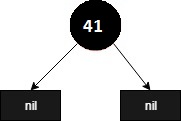
\includegraphics[width=\linewidth]{1.jpg}
     	\caption{Inserting 41}
   	\end{subfigure}
  	\begin{subfigure}[p]{0.4\linewidth}
    	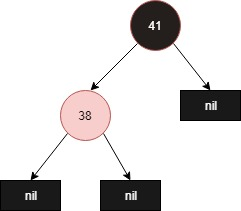
\includegraphics[width=\linewidth]{2.jpg}
    	\caption{Inserting 38}
  	\end{subfigure}

  	\centering
   	\begin{subfigure}[p]{0.4\linewidth}
    	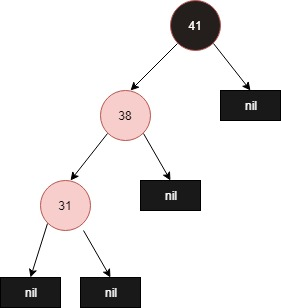
\includegraphics[width=\linewidth]{3-1.jpg}
     	\caption{Inserting 31}
   	\end{subfigure}
  	\begin{subfigure}[p]{0.4\linewidth}
    	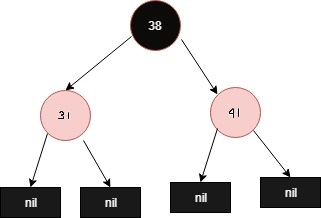
\includegraphics[width=\linewidth]{3-2.jpg}
    	\caption{Re-balancing}
  	\end{subfigure}

   	\begin{subfigure}[p]{0.4\linewidth}
    	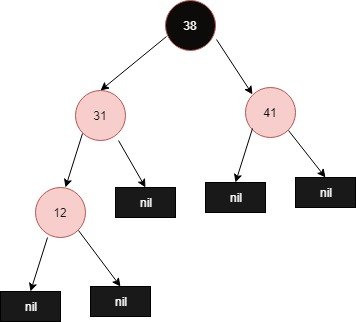
\includegraphics[width=\linewidth]{4-1.jpg}
     	\caption{Inserting 12}
   	\end{subfigure}
  	\begin{subfigure}[p]{0.4\linewidth}
    	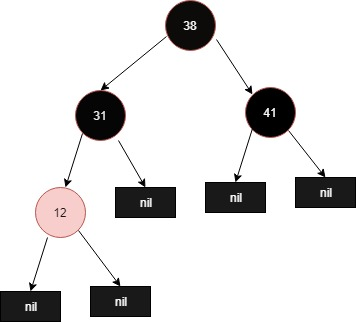
\includegraphics[width=\linewidth]{4-2.jpg}
    	\caption{Re-balancing}
  	\end{subfigure}
\end{figure}
\begin{figure}

   	\begin{subfigure}[p]{0.4\linewidth}
    	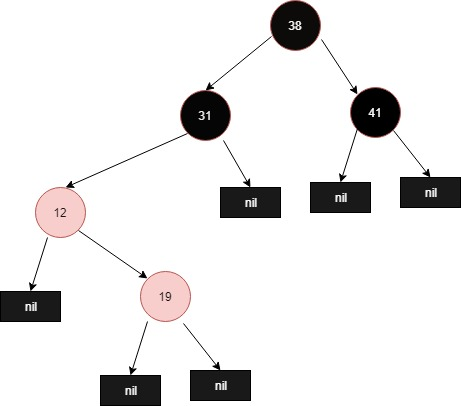
\includegraphics[width=\linewidth]{5-1.jpg}
     	\caption{Inserting 12}
   	\end{subfigure}
  	\begin{subfigure}[p]{0.4\linewidth}
    	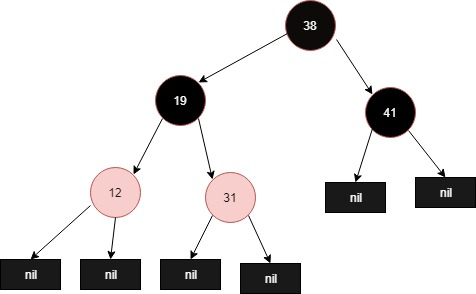
\includegraphics[width=\linewidth]{5-2.jpg}
    	\caption{Re-balancing}
  	\end{subfigure}

   	\begin{subfigure}[p]{0.4\linewidth}
    	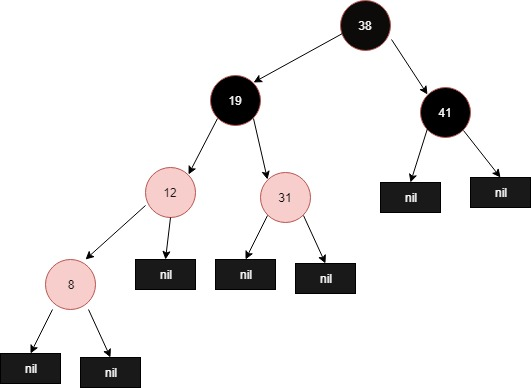
\includegraphics[width=\linewidth]{6-1.jpg}
     	\caption{Inserting 12}
   	\end{subfigure}
  	\begin{subfigure}[p]{0.4\linewidth}
    	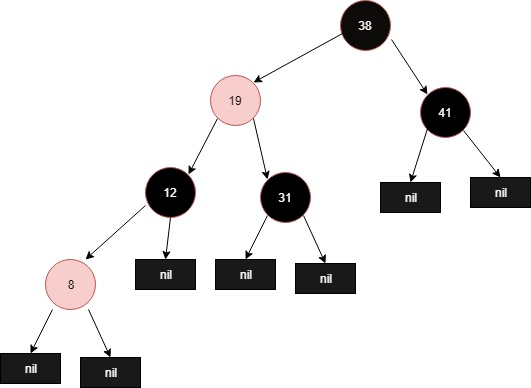
\includegraphics[width=\linewidth]{6-2.jpg}
    	\caption{Re-balancing}
  	\end{subfigure}

\end{figure}

\newpage
\newpage
\newpage
\newpage
\section{Question 13.4-3}
In Exercise 13.3-2, you found the red-black tree that results from successively inserting the keys 41, 38, 31, 12, 19, 8 into an initially empty tree. Now show the red-black trees that result from the successive deletion of the keys in the order 8, 12, 19, 31, 38, 41. \\
\noindent\rule{2cm}{0.4pt} \\


\section{Question 14.1-3}
Show how OS-SELECT(T.root, 10) operates on the red-black tree T of Figure 14.1 \\
\noindent\rule{2cm}{0.4pt} \\

It may be useful to have the code for OS-SELECT(x, i) below to walk through 
\begin{verbatim}
OS-SELECT(x,i)
   r = x.left.size+ 1
   if i == r
     return x
   elseif i < r
     return OS-SELECT(x.left, i)
   else return OS-SELECT(x.right, i - r)
\end{verbatim} 

First we calculate the rank of the root. $r = 12 + 1 = 13$. since $i = 10$, and $10 < 13$, we recursively call OS-SELECT(T.root.left, 10). \\
Now we calculate the rank of the current subtree root. $r = 7 + 1 = 8$. since $8 < 10$, we call OS-SELECT(x.right, 2). \\
Now we are at the node with a key =  21, and we calculate its rank. $r = 2 + 1 = 3$. since $i < r$, we take the left subtree, and call OS-SELECT(x.left, 2) \\
Now we are at the node with key = 19, where $i = 2$, and rank $r = 0 + 1 = 1$.  since $i > r$, we make the call OS-SELECT(x.right, 1). \\
Now we are at node key = 20.  $r = 0 + 1 = 1$ and $i = 1$ thus, since $i == r$, we have our 10th smallest node, which is node where key = 20.

\section{Question 14.1-5}
Given an element $x$ in an $n$-node order-statistic tree and a natural number $i$, how can we determine the $i$th successor of $x$ in linear order of the tree in $\mathcal{O}(\lg n)$ time? \\
\noindent\rule{2cm}{0.4pt} \\

determining the $i$th successor of a node x is similar to determining $i$th smallest element, except that we pretend that $x$ is the smallest node in the tree.  So determining the $i$th successor in $x$ is essentially taking the rank of $x$ and adding it to the $i$th smallest element greater than $x$.  So for example, if the rank of $x$ is 4, then finding the 3rd successor of $x$ is equivalent to OS-SELECT(T.root, x.rank + 3) = OS-SELECT(T.root, 7). or to word this generally, we can use the pseudocode function from the book OS-RANK(T,x) and plug it into our OS-SELECT function.
\begin{verbatim}
OS-SELECT(T.root, OS-RANK(T, x) + i)
\end{verbatim}


\section{Question 14.1-6}
Observe that whenever we reference the size attribute of a node in either OS-SELECT or OS-RANK, we use it only to compute a rank.  Accordingly, suppose we store in each node its rank in the subree of which it is the root. Show how to maintain this information during insertion and deletion. (Remember that these two operations can cause rotations). \\
\noindent\rule{2cm}{0.4pt} \\


\section{Question 14.1-7}
Show how to use an order-statistic tree to count the number of inversions (see problem 2-4) in an array of size $n$ in time $\mathcal{O}(n \lg n)$  \\ 
\noindent\rule{2cm}{0.4pt} \\

Problem 2-4 states: \\
Let $A[1..n]$ be an array of $n$ distinct numbers. If $i < j$ and $A[i] > A[j]$, then the pair $(i,j)$ is called an inversion of A. \\ \\





\end{document}
